\documentclass[11pt,a4paper]{article}
\usepackage[T1]{fontenc}
\usepackage[utf8]{inputenc}
\usepackage{lmodern}
\usepackage[margin=2.5cm]{geometry}
\usepackage{microtype}
\usepackage{amsmath}
\usepackage{booktabs}
\usepackage{graphicx}
\usepackage{caption}
\usepackage{threeparttable}
\usepackage{tabularx}
\usepackage[authoryear,round]{natbib}
\usepackage{xcolor}
\usepackage[colorlinks=true,linkcolor=blue!50!black,citecolor=blue!50!black,urlcolor=blue!50!black]{hyperref}
\usepackage{setspace}
\usepackage[section]{placeins}
\setstretch{1.08}
\captionsetup{font=small,labelfont=bf,margin=0.5cm}
\graphicspath{{../output/figures/}}
\newcommand{\figwidth}{0.92\textwidth}

\title{\textbf{Sanctions and Russian Invention}\\[0.3em]
\large Results with official IPC codes, industry-level designs and input exposure}
\author{Fyodor Shafranov\thanks{LMU Munich. Work in progress; not for citation. Every number comes from the
replication package in this repository (\texttt{run\_all.sh}); design rules are logged in
\texttt{notes/data\_decisions.md} and were fixed before the corresponding estimates were seen. Detailed notes:
\texttt{notes/13}--\texttt{15}. Some references below were not re-verified for this draft.}}
\date{20 November 2026 --- results report (supersedes the 12 November draft)}

\begin{document}
\maketitle

\begin{abstract}
\noindent
After February 2022 the European Union banned the export to Russia of products that made up about half of Russia's
pre-war Western imports of manufactured goods. I ask whether Russian domestic invention moved \emph{into} the banned
technologies (import substitution) or fell where Western inputs were cut. All Russian invention patents filed since
1994 now carry their official IPC codes, downloaded from the Rospatent search platform. Across 35 WIPO technology
fields, one standard deviation more ban coverage is associated with about 9\% fewer domestic patents after 2022
($-0.096$ log points, 95\% CI $[-0.150, -0.042]$, randomization $p=0.0015$). The pre-period passes a small-cluster bootstrap test
($p=0.51$), the estimate is unchanged by pre-war controls, and HonestDiD bounds show robustness to a continuation of
the mild pre-2022 slope. The result replicates in a different design that assigns patents to 55 manufacturing
industries and measures ban coverage directly from trade data ($-0.077$ log points, $p=0.002$, flat pre-period), and with
input-based exposure built from US and Russian input-output tables. The decline is concentrated in research
institutes and universities, operates between broad technology fields and industry branches rather than within them,
and is tied to what was banned, not to reliance on Western inputs in general. The narrower 2014 sanctions show the
opposite pattern: invention moved into the restricted dual-use technologies.
\end{abstract}

\section{Question and design}

Sanctions can raise domestic invention in the banned technologies (substitution: the domestic return to inventing
what can no longer be bought rises) or lower it (complementarity: domestic research needs imported equipment,
components and knowledge). The 2022 EU export bans give a large, dated, sender-defined shock whose intensity differs
across technologies. The main design compares technology fields (or industries) that lost more of their Western
imports to the bans with those that lost less, before and after 2022:
\begin{equation}
  E[P_{ft}] = \exp\!\big(\beta\,\mathrm{Ban}_f \times \mathrm{Post}_t + \alpha_f + \gamma_t\big),
  \label{eq:main}
\end{equation}
where $P_{ft}$ counts domestic invention patents filed in field $f$ in year $t$ (fractional counts over a patent's
fields; mass filers dropped), $\mathrm{Ban}_f$ is the share of the field's 2019--21 Western imports banned by the EU
by the end of 2023 (z-scored), and $\alpha_f$, $\gamma_t$ are field and year fixed effects. Estimation is by Poisson
pseudo-maximum likelihood (PPML), 2015--2025, with standard errors clustered by field. The event-study version
replaces $\mathrm{Post}_t$ with year dummies (base 2021). The treatment is continuous, so $\beta$ compares more- with
less-exposed fields; there is no untreated group. The measure is a shift-share exposure in the sense of
\citet{BorusyakHullJaravel2022}: product-level bans (shocks) weighted by each field's pre-war import composition
(shares), as in the industry exposure of \citet{EgorovEtAl2026}.

\section{Data}

\begin{itemize}\setlength\itemsep{0.15em}
  \item \textbf{Patents.} The Rospatent register of granted inventions, with official IPC codes for every patent from
  the Rospatent search-platform API (531,365 documents, filing years 1994--2026, 98--99.5\% of the register in
  2015--2025). Official codes replace the title-based classifier of the earlier draft. About 15,000--18,000 domestic
  patents per filing year; 2025 filings are still incomplete because of the grant lag.
  \item \textbf{Bans.} All 35 consolidated versions of Council Regulation (EU) 833/2014: export-ban annexes, customs
  codes converted to HS 2007 six-digit products, share of each product banned, by date.
  \item \textbf{Imports.} Russia's imports by product and partner from CEPII BACI \citep{GaulierZignago2010}; ``West''
  is the 2022 sanctions coalition.
  \item \textbf{Products to technologies.} Two independent maps: an industry map (HS $\to$ ISIC $\to$ industry
  $\to$ field, using the \citealp{DornerHarhoff2018} table) and a product-name map (a text classifier applied to
  customs descriptions). They correlate 0.7 across fields.
  \item \textbf{Industry designs.} Patents to NACE 3-digit industries with the Dorner--Harhoff IPC-subclass $\to$
  industry table; input structure from the BEA 2017 detailed use table and from Rosstat's 2021 basic input-output
  tables (recovered from the Internet Archive; the live links are dead).
  \item \textbf{2014.} The EU oil-equipment list (Annex II) and the Commission's dual-use correlation table
  (1 April 2014) for the dual-use restrictions.
\end{itemize}
The bans bite: by the end of 2023 they cover 49\% of Russia's 2019--21 Western manufactured imports, one standard
deviation more coverage predicts 31--48 log points lower Western imports into the field in 2023, and China did not
replace more in banned fields.

\section{Main result: 35 technology fields}

Figure~\ref{fig:main} shows the event study with both maps and confidence intervals from a pairs cluster
bootstrap-t over fields, which is reliable with few clusters. Before 2022 no coefficient excludes zero; from 2022 the
more exposed fields fall behind: $-0.045$, $-0.094$, $-0.091$, $-0.089$ log points per standard deviation in
2022--2025 (industry map). Table~\ref{tab:main} collects the pooled estimates.

\begin{figure}[ht]
\centering
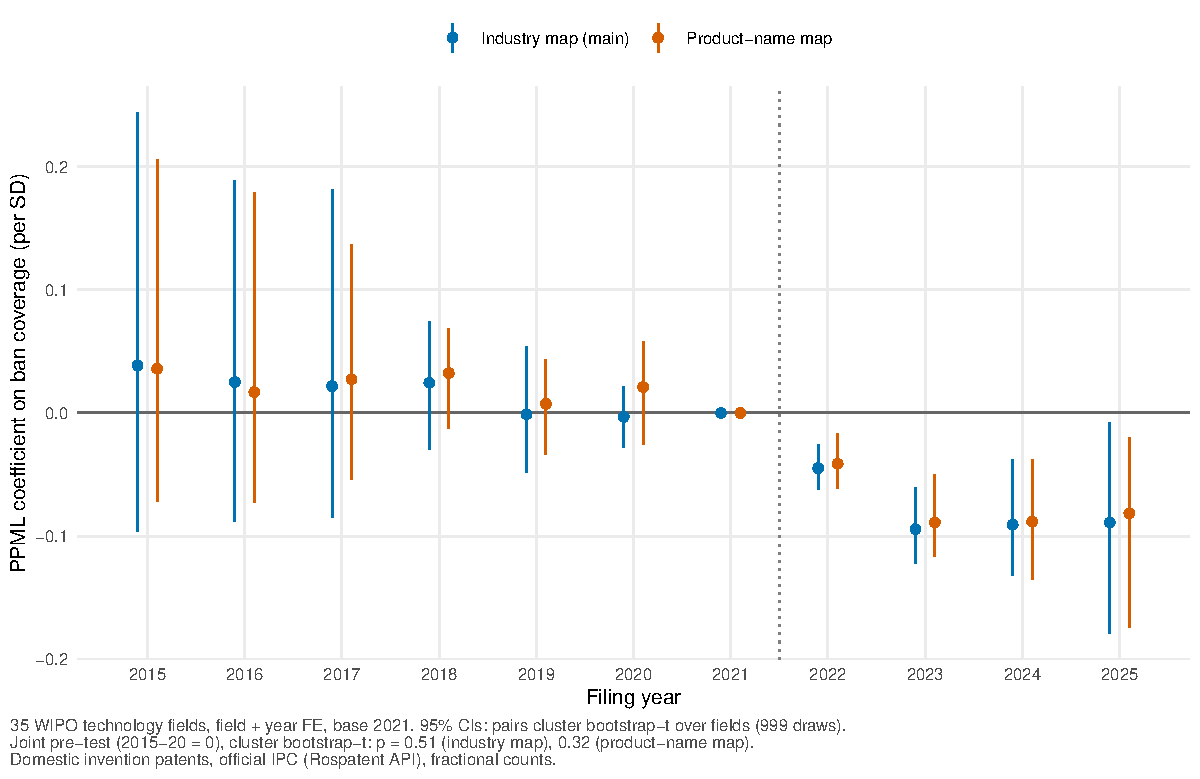
\includegraphics[width=0.82\textwidth]{fig38b_fields_official_es_boot.pdf}
\caption{Domestic invention patents by technology field and EU ban coverage. PPML, field and year fixed effects,
base 2021, coefficient per standard deviation of coverage. 95\% CIs from a pairs cluster bootstrap-t (999 draws).}
\label{fig:main}
\end{figure}

\begin{table}[ht]
\centering
\begin{threeparttable}
\caption{Pooled effect of ban coverage on domestic patents, 35 fields}
\label{tab:main}
\small
\begin{tabular}{lcc}
\toprule
Specification & Estimate (per SD) & 95\% CI / $p$ \\
\midrule
Main: field + year FE, industry map & $-0.096$ & $[-0.150, -0.042]$; RI $p=0.0015$ \\
Product-name map & $-0.096$ & $[-0.151, -0.041]$ \\
Sector $\times$ year FE (WIPO's 5 sectors) & $-0.096$ & $[-0.155, -0.036]$ \\
Pre-war controls $\times$ year (6 versions) & $-0.093$ to $-0.115$ & all $p \le 0.001$ \\
Leave one field out (35 estimates) & $-0.072$ to $-0.107$ & all CIs below 0 \\
Without the 5 life-science fields & $-0.049$ & $[-0.096, -0.002]$ \\
Top vs bottom third of fields (binary) & $-0.228$ & SE 0.071 \\
\bottomrule
\end{tabular}
\begin{tablenotes}\footnotesize
\item PPML, 2015--2025. RI: randomization inference, coverage permuted across fields. Pre-war controls (each alone and all four together): university
share of patents, Western share of total imports, foreign-holder share, size (2015--19), z-scored, interacted with
year dummies.
\end{tablenotes}
\end{threeparttable}
\end{table}

\paragraph{Size.} $-0.096$ log points is about $-9$\% per standard deviation (about 15 percentage points) of ban
coverage, relative to less exposed fields. In the raw data a good part of the gap comes from growth in the least
exposed fields, mostly the life sciences, where patenting by universities rose after 2022 (Figure~\ref{fig:raw}).
Dropping the five life-science fields halves the estimate.

\begin{figure}[ht]
\centering
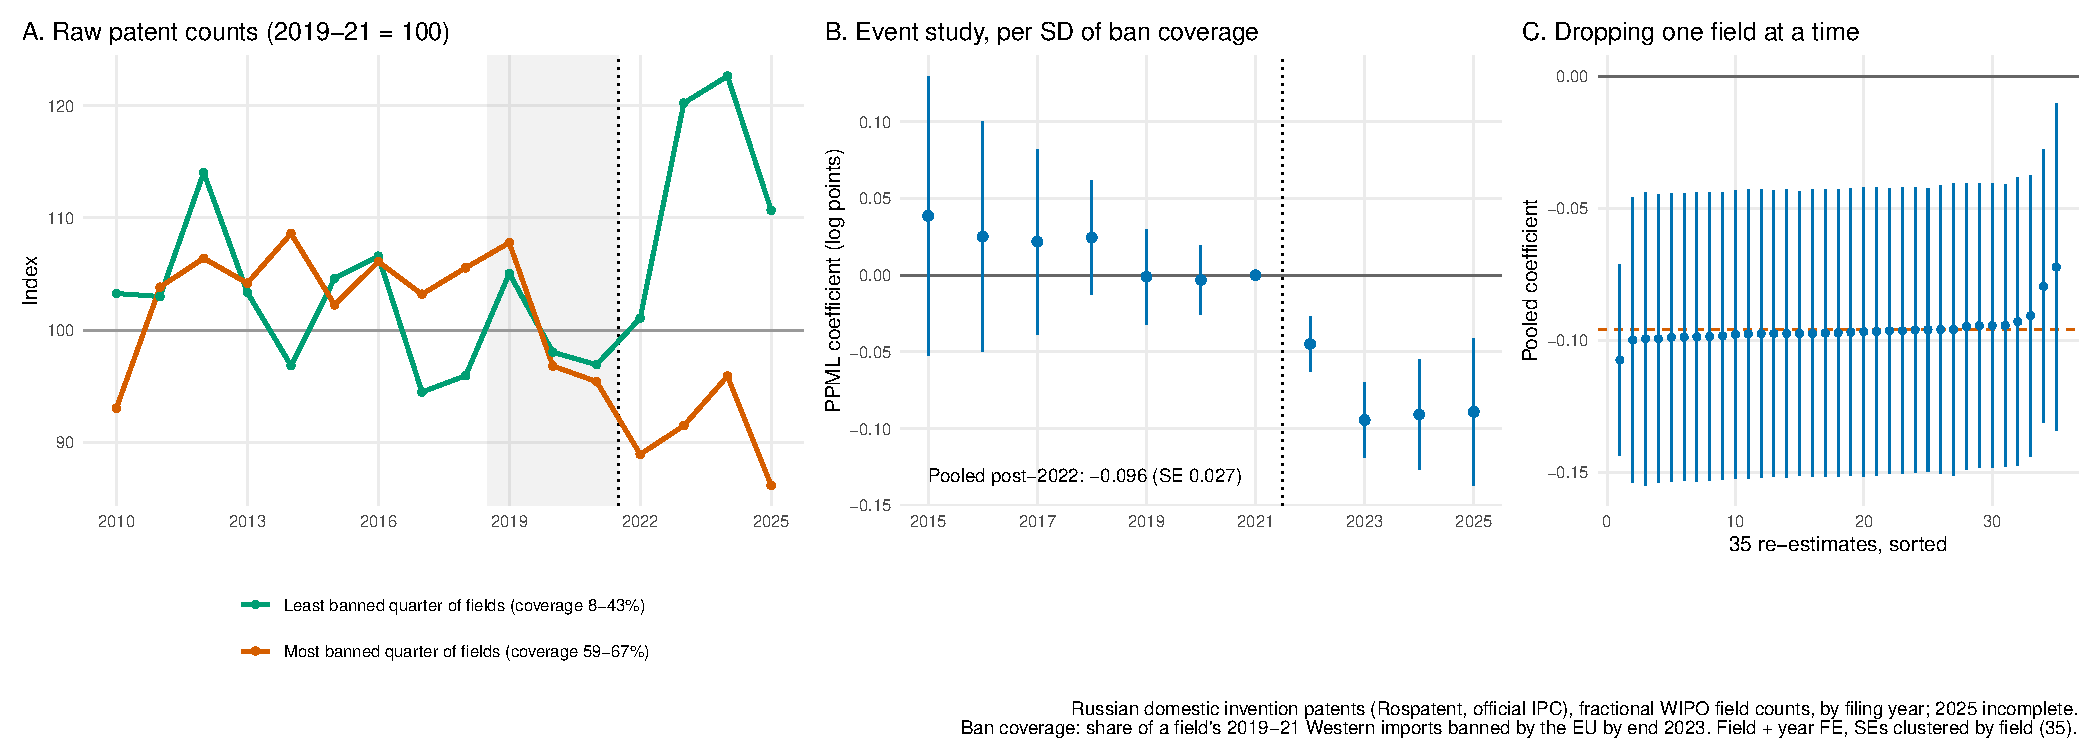
\includegraphics[width=\textwidth]{fig48_summary.pdf}
\caption{(A) Raw patents in the most and least exposed quarters of fields (2019--21 $=100$). (B) Event study.
(C) Pooled estimate dropping one field at a time.}
\label{fig:raw}
\end{figure}

\paragraph{Who.} By holder type (pooled, industry map): research institutes $-0.126$, individuals $-0.125$,
universities $-0.103$ (all CIs below zero), firms $-0.039$ (CI $[-0.108, 0.030]$). Public research organisations
fall by 0.075 more than firms ($p=0.006$). The decline is concentrated where research depends on imported equipment
and international links, not in firms' product development.

\section{Pre-trends}

Each pre-period coefficient includes zero, but they slope gently down (from $+0.04$ in 2015 to 0 in 2020), and the
standard clustered Wald test of all six rejects ($p=0.02$; product-name map $p=0.001$). Four checks:
\begin{enumerate}\setlength\itemsep{0.15em}
  \item \textbf{Small-cluster inference.} With 35 clusters, cluster-robust joint tests over-reject. A pairs cluster
  bootstrap-t gives $p=0.51$ (industry map) and $0.32$ (product-name map); a wild cluster restricted bootstrap on the
  OLS version gives $0.28$. Across all pre-war control sets the bootstrap $p$ is $0.23$--$0.63$.
  \item \textbf{Linear trend and placebo.} A linear pre-trend is $-0.007$ per year ($p=0.40$); a placebo break in
  2018 on 2015--2021 data gives nothing ($p=0.44$).
  \item \textbf{Pre-war controls.} University share, Western import dependence, foreign presence and size, each
  $\times$ year, leave the estimate at $-0.09$ to $-0.12$ (Figure~\ref{fig:controls} in the appendix).
  \item \textbf{HonestDiD} \citep{RambachanRoth2023}. If the pre-period slope continued linearly after 2021, the
  average 2022--25 effect is still $[-0.077, -0.034]$. Under relative-magnitude restrictions the effect survives
  violations up to 0.75 (average effect) and 1.0 (2023) times the largest pre-period year-to-year change with the
  industry map, 0.5--0.75 with the product-name map (Figure~\ref{fig:honest}).
\end{enumerate}
A long window (2005--2025, base 2013) shows that the later-banned fields gained ground before 2014, peaked in 2014,
drifted down in 2015--2021 and dropped in 2022. Against the 2005--13 baseline, 2014--21 is on average unchanged
($+0.005$, $p=0.83$) and 2022+ is $-0.098$ ($p=0.047$). The 2015--21 drift is not early treatment through the 2014
dual-use restrictions (Section~\ref{sec:2014}).

\begin{figure}[ht]
\centering
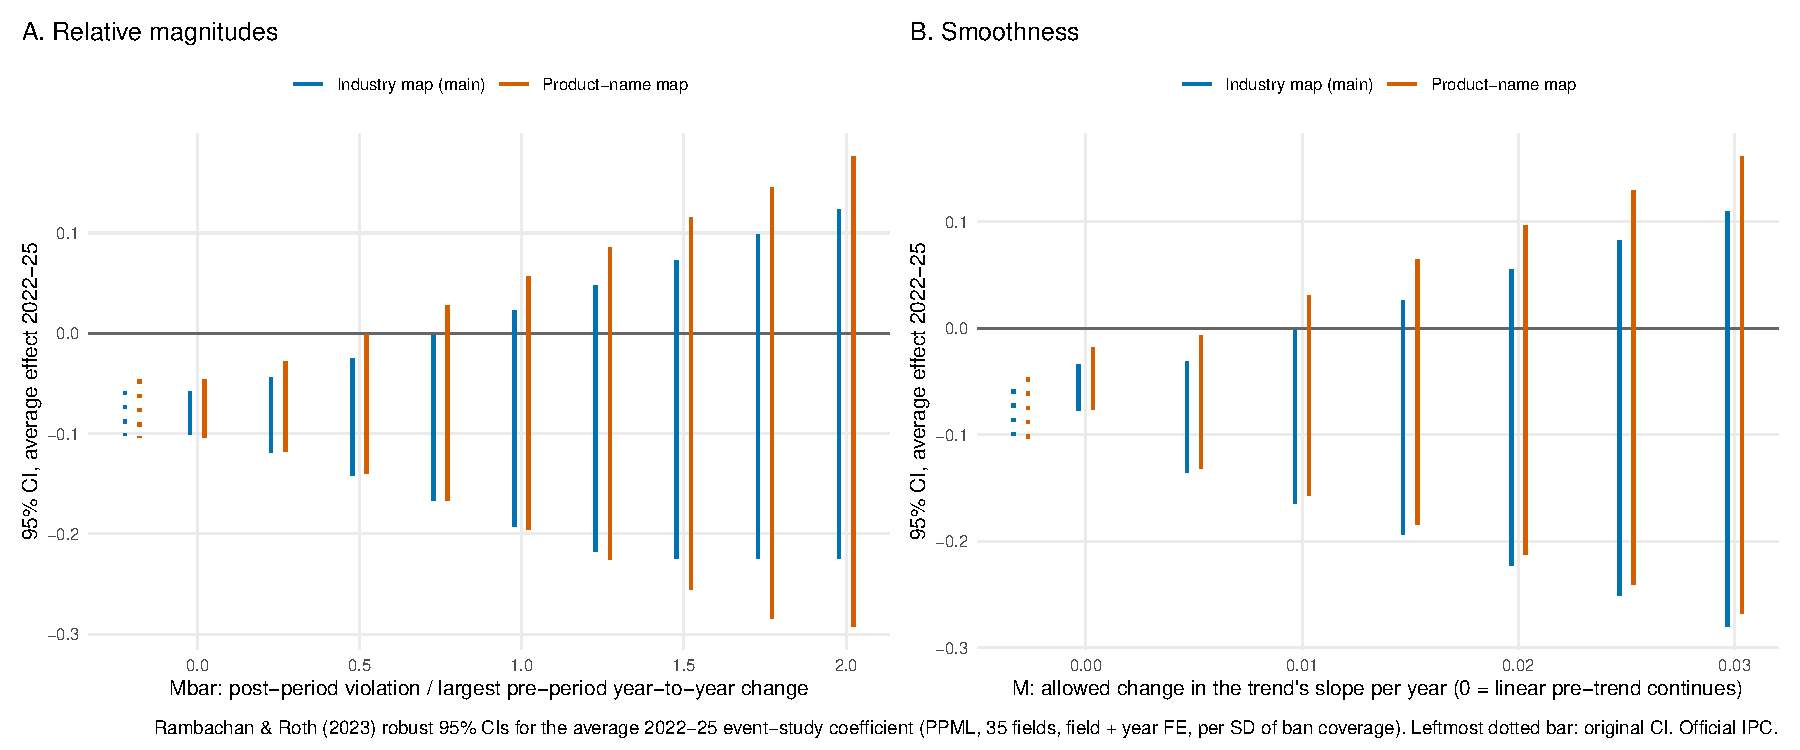
\includegraphics[width=\textwidth]{fig53_honestdid.pdf}
\caption{HonestDiD robust 95\% CIs for the average 2022--25 coefficient: (A) relative magnitudes, (B) smoothness.}
\label{fig:honest}
\end{figure}

\section{Industries instead of technology fields}

The field design needs a product $\to$ technology link on the treatment side, which attenuates the estimate if noisy.
The industry design moves the link to the outcome side, where errors mostly cost precision: patents are assigned to
55 NACE 3-digit manufacturing industries through their official IPC subclass (Dorner--Harhoff table, 99.7\% of
patents covered), and ban coverage is the banned share of the industry's 2019--21 Western imports (HS $\to$ ISIC,
repair and installation links dropped). Coverage varies much more across industries (SD 32 percentage points) than
across fields (15). Pharmaceuticals have almost zero coverage because medicines were exempt.

\begin{table}[ht]
\centering
\begin{threeparttable}
\caption{Industry-level design with output exposure, 55 NACE 3-digit manufacturing industries}
\label{tab:industry}
\small
\begin{tabular}{lccc}
\toprule
Fixed effects & Estimate (SE) & RI $p$ & Pre-test $p$ (Wald / bootstrap) \\
\midrule
industry + year & $-0.077$ (0.026) & 0.002 & 0.59 / 0.85 \\
industry + division $\times$ year & $-0.019$ (0.025) & 0.28 & 0.02 / 0.60 \\
OLS $\log(1+n)$, industry + year & $-0.025$ (0.014) & -- & -- \\
\bottomrule
\end{tabular}
\begin{tablenotes}\footnotesize
\item PPML unless stated, 2015--2025, per SD of exposure, SEs clustered by industry. RI: coverage permuted across
industries (1,000 draws). Pre-test: joint test of the 2015--2020 coefficients; bootstrap = pairs cluster bootstrap-t.
\end{tablenotes}
\end{threeparttable}
\end{table}

\begin{figure}[ht]
\centering
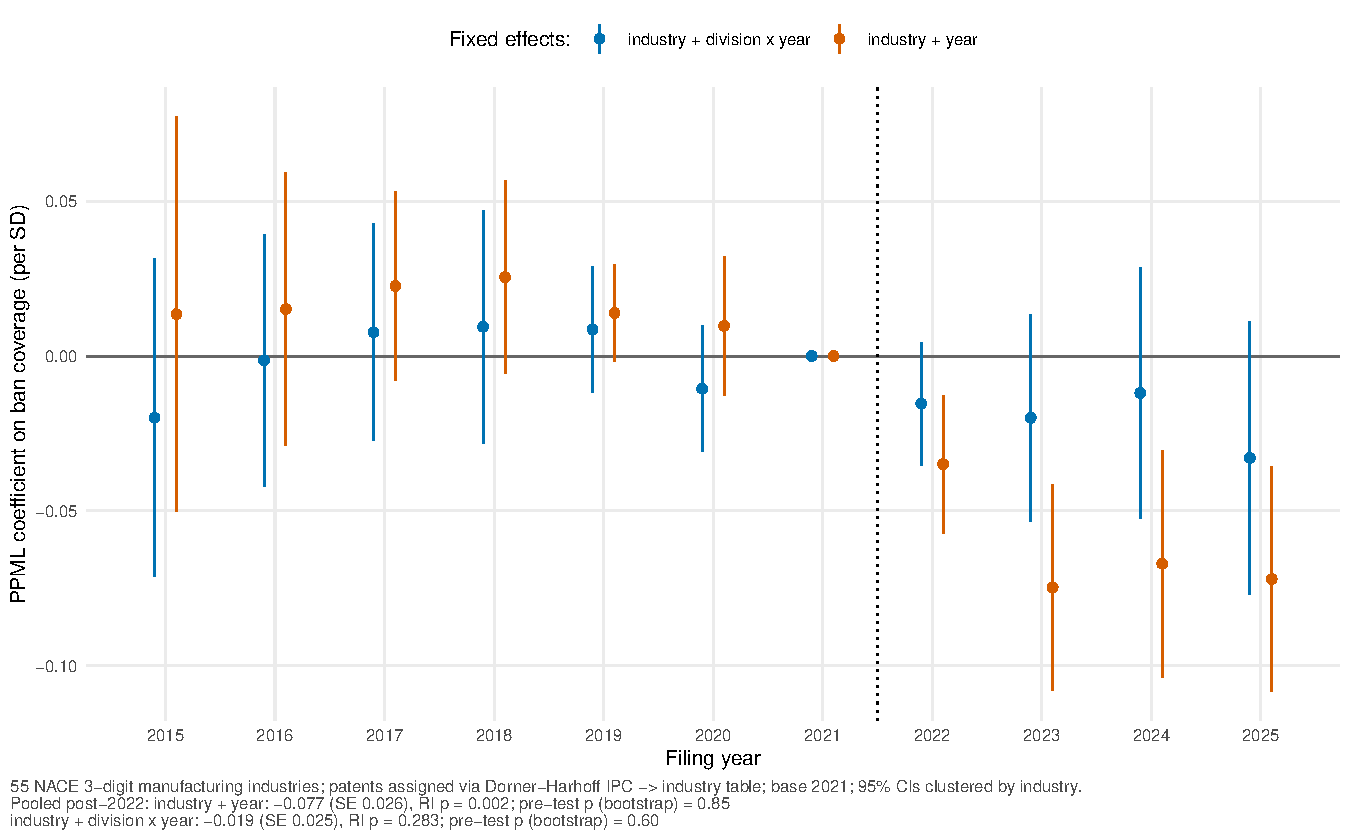
\includegraphics[width=0.82\textwidth]{fig57_industry_es.pdf}
\caption{Industry-level event study (output exposure), with industry + year and industry + division $\times$ year
fixed effects.}
\label{fig:industry}
\end{figure}

Two findings (Table~\ref{tab:industry}, Figure~\ref{fig:industry}):
\begin{enumerate}\setlength\itemsep{0.15em}
  \item \textbf{The result replicates} with a different link on both sides: $-0.077$ per standard deviation, with a
  flat pre-period that needs no correction (Wald $p=0.59$, bootstrap $0.85$). OLS on $\log(1+n)$, which weights
  small industries as much as large ones, gives a smaller, marginal $-0.025$ ($p=0.07$).
  \item \textbf{It operates between branches.} Within 2-digit divisions there is no effect ($-0.019$). The same holds
  for IPC subclasses within technology fields (Section~\ref{sec:subclass}). Without pharmaceuticals the industry
  estimate is $-0.056$ with a CI that includes zero.
\end{enumerate}

\section{Input-based exposure: input-output methods}
\label{sec:io}

\paragraph{What changes.} Output exposure measures the banned share of what an industry \emph{makes}: Russia's
imports of the industry's own products. It does not see what the industry \emph{uses}. Pharmaceuticals, for
example, have almost no output exposure because medicines were exempt, although some of their laboratory
instruments and process machinery were banned. Input exposure weights banned products by how much each industry
buys of them, which is closer to the firm-level measure of \citet{EgorovEtAl2026} (the share of a firm's own pre-war
imports in later-sanctioned products). The two measures correspond to two channels: lost Western products in the
industry's own market (output) and lost Western inputs (input).

\paragraph{US input weights (BEA).} The BEA 2017 detailed use table records purchases of about 400 commodities by
about 400 industries. BEA codes are linked to NAICS 2017 (BEA's own list), NAICS to ISIC Rev.~4 (R package
\texttt{concordance}) and ISIC to our NACE 3-digit units. Each commodity $c$ gets a ban share $b_c$: the banned share
(end-2023) of Russia's 2019--21 Western imports in its product group. Input exposure of industry $j$ is
\begin{equation}
  \mathrm{In}_j^{\mathrm{BEA}} = \frac{\sum_c U_{cj}\, b_c}{\sum_c U_{cj}},
\end{equation}
where $U_{cj}$ is $j$'s use of manufactured commodity $c$. A variant excludes the industry's own product group. The
US table is a proxy for how industries combine inputs; its advantage is detail (about 230 manufacturing industries).

\paragraph{Russian input weights (Rosstat).} Rosstat's basic input-output tables for 2021 (taken down from the
Rosstat site; recovered from the Internet Archive) contain a use table of \emph{imported} products by industry
(sheet \textit{M-imp}) and of domestic products (\textit{M-otech}), 124 manufactured product rows (OKPD~2) and 46 manufacturing industry
columns. With $M_{pj}$ and $D_{pj}$ the imported and domestic use of product $p$ by industry $j$, $\omega_p$ the
Western share of Russia's 2019--21 imports of $p$ and $b_p$ the banned share of those Western imports:
\begin{align}
  \mathrm{Dep}_j &= \frac{\sum_p M_{pj}\,\omega_p\, b_p}{\sum_p (M_{pj} + D_{pj})}
    && \text{banned Western inputs / all inputs (main)},\\
  \mathrm{Sh}_j &= \frac{\sum_p M_{pj}\,\omega_p\, b_p}{\sum_p M_{pj}\,\omega_p}
    && \text{banned share of Western imported inputs},\\
  \mathrm{West}_j &= \frac{\sum_p M_{pj}\,\omega_p}{\sum_p (M_{pj} + D_{pj})}
    && \text{Western import dependence regardless of bans}.
\end{align}
These are Russia's own 2021 input weights, by origin, for the year before the bans. In 2021 electronics bought 19\%
of its manufactured inputs from the West and 65\% of those were later banned ($\mathrm{Dep}=0.12$); pharmaceuticals
bought 32\% from the West but only 9\% of that was banned ($\mathrm{Dep}=0.027$).

\paragraph{Inference.} Rosstat publishes the using industries for electronics, electrical equipment, machinery,
motor vehicles and other transport only at the 2-digit level, in the use table and in the symmetric tables alike.
NACE 3-digit industries inside one column therefore share one value, and exposure varies over only 29 columns that
contain sample industries. Standard errors are clustered by column and randomization inference permutes exposure
across columns. The BEA measure varies across all 55 industries.

\begin{table}[ht]
\centering
\begin{threeparttable}
\caption{Input-based exposure, 55 NACE 3-digit manufacturing industries}
\label{tab:io}
\footnotesize
\setlength{\tabcolsep}{4pt}
\begin{tabular}{>{\raggedright\arraybackslash}p{2.6cm}>{\raggedright\arraybackslash}p{5.0cm}ccc}
\toprule
Input weights & Specification & Estimate (SE) & RI $p$ & Pre-test $p$ \\
\midrule
BEA (US, 2017) & $\mathrm{In}^{\mathrm{BEA}}$ alone & $-0.067$ (0.009) & 0.003 & 0.10 \\
 & excluding own products & $-0.058$ (0.009) & 0.025 & 0.07 \\
 & with output exposure: input & $-0.050$ (0.023) & 0.14 & 0.16 \\
 & \hspace{2.45cm}output & $-0.030$ (0.039) & 0.42 & 0.59 \\
Rosstat (Russia, 2021) & $\mathrm{Dep}$ alone & $-0.059$ (0.018) & 0.063 & 0.24 \\
 & $\mathrm{Sh}$ alone & $-0.069$ (0.016) & 0.045 & 0.83 \\
 & $\mathrm{Dep}$ with $\mathrm{West}$: Dep & $-0.066$ (0.009) & 0.15 & 0.26 \\
 & \hspace{1.95cm}West & $+0.040$ (0.023) & 0.38 & 0.91 \\
 & $\mathrm{Dep}$ with output exposure: Dep & $-0.034$ (0.021) & 0.14 & 0.31 \\
 & \hspace{3.1cm}output & $-0.061$ (0.031) & -- & 0.91 \\
\bottomrule
\end{tabular}
\begin{tablenotes}\footnotesize
\item PPML, industry + year FE, 2015--2025, per SD of exposure. SEs clustered by industry (BEA) or by the 29
Rosstat columns (Rosstat). Pre-test: joint test of the 2015--2020 coefficients, pairs cluster bootstrap-t.
\end{tablenotes}
\end{threeparttable}
\end{table}

\paragraph{Results.} Four findings (Table~\ref{tab:io}, Figures~\ref{fig:bea} and \ref{fig:rosstat}):
\begin{enumerate}\setlength\itemsep{0.15em}
  \item \textbf{Same size.} Input exposure gives $-0.06$ to $-0.07$ per standard deviation with either set of
  weights, the same as output exposure. Excluding the industry's own products barely changes the BEA estimate.
  \item \textbf{Channels not separable.} With BEA weights the input measure keeps its effect when output exposure is
  added ($-0.050$) and output loses it; with Rosstat weights it is the reverse. With 55 industries and measures that
  correlate 0.4--0.6, lost inputs and lost Western products in the industry's own market cannot be told apart.
  \item \textbf{Bans, not Western ties.} Controlling for Western import dependence regardless of bans leaves the
  banned-input effect at $-0.066$; dependence itself is not negative. Splitting Western inputs into banned
  ($\mathrm{Dep}$) and unbanned ($\mathrm{West}-\mathrm{Dep}$) parts, which are uncorrelated (0.02), unbanned access
  has no effect once pharmaceuticals and medical goods are dropped ($+0.001$, $p=0.87$), while the banned part stays
  at $-0.04$ to $-0.05$ in every sample. The positive unbanned coefficient in the full sample is pharmaceuticals:
  high Western reliance, exempt from the bans, and university-driven growth.
  \item \textbf{Precision.} The Rosstat estimates are marginal under randomization inference ($p=0.045$--$0.15$)
  because exposure varies over only 29 columns. They confirm the direction and size of the main result rather than
  stand on their own.
\end{enumerate}

\begin{figure}[ht]
\centering
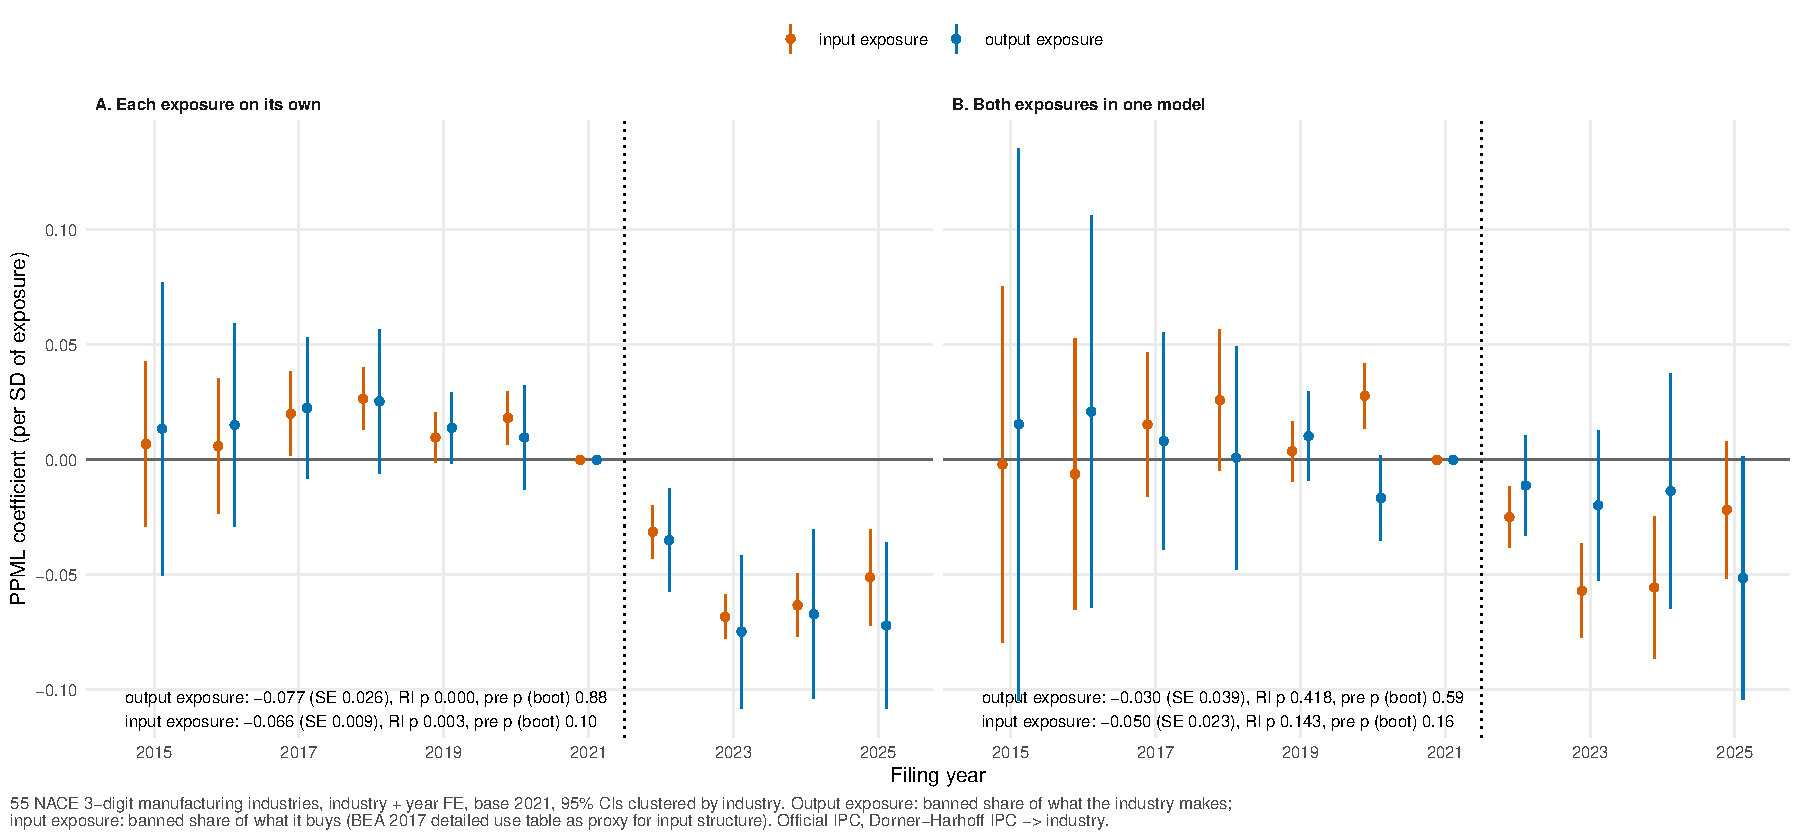
\includegraphics[width=\textwidth]{fig58_input_exposure_es.pdf}
\caption{Output vs input exposure (BEA weights): each alone (A) and both in one model (B).}
\label{fig:bea}
\end{figure}

\begin{figure}[ht]
\centering
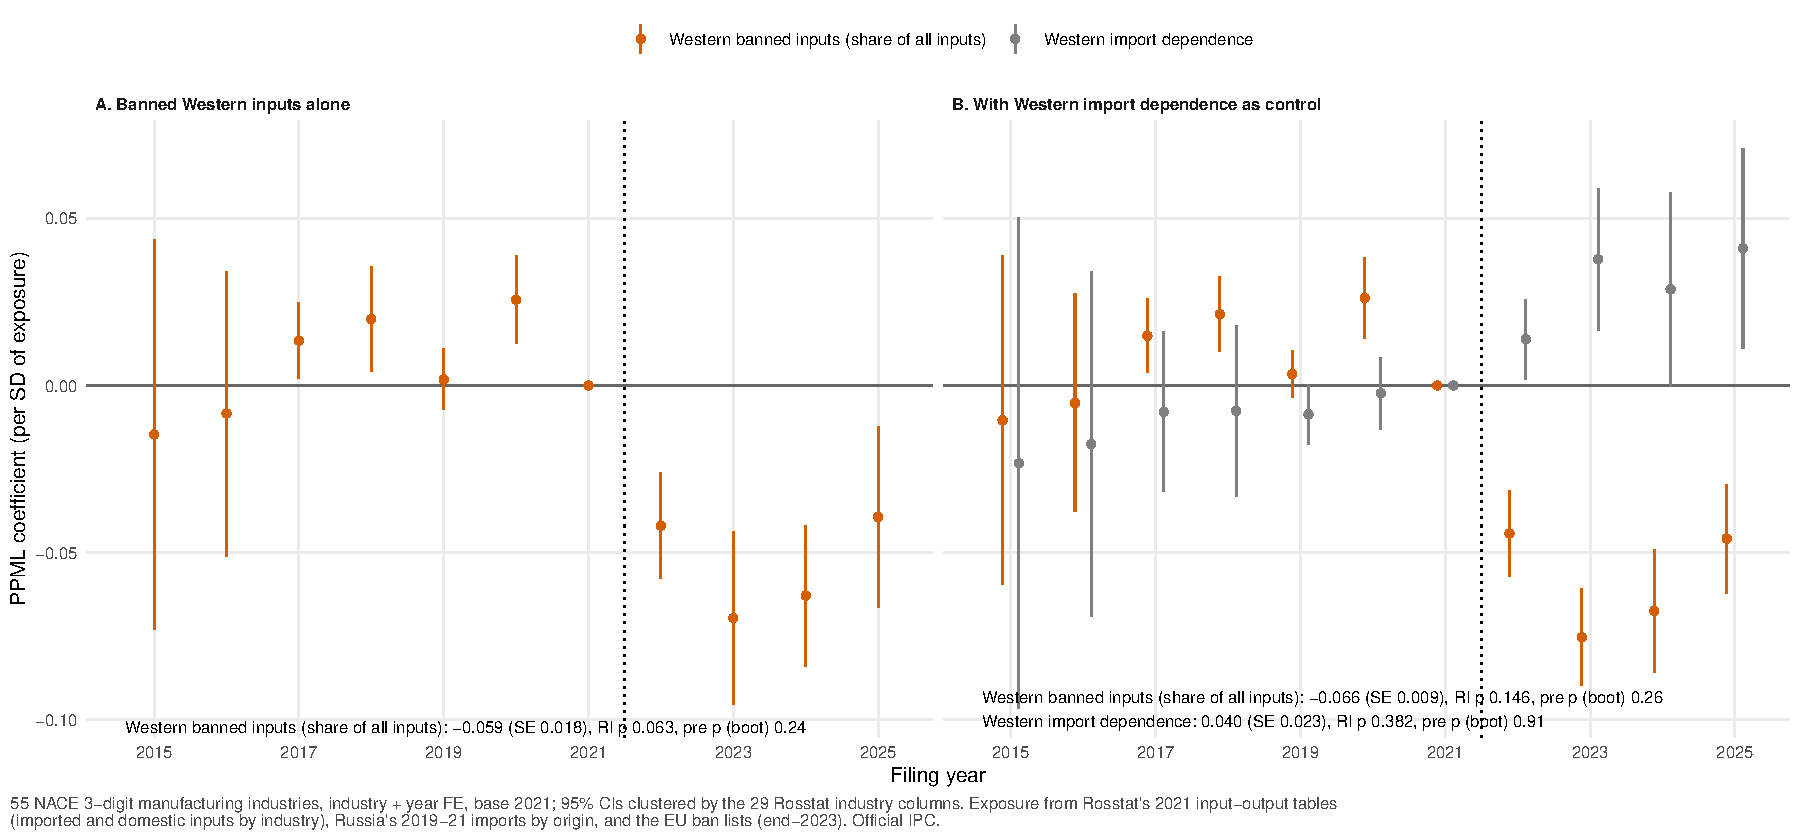
\includegraphics[width=\textwidth]{fig59_rosstat_input_es.pdf}
\caption{Banned Western inputs from Rosstat's 2021 input-output tables ($\mathrm{Dep}$), alone (A) and with Western
import dependence ($\mathrm{West}$) as a control (B). 95\% CIs clustered by Rosstat column.}
\label{fig:rosstat}
\end{figure}

\section{Finer units: IPC subclasses}
\label{sec:subclass}

Across about 280 IPC subclasses (subclass + year FE) the drop after 2022 is present, but PPML versions show
a pre-existing downward slope; only OLS on $\log(1+n)$ has a flat pre-period, and only with the industry map. Within
fields (subclass + field $\times$ year FE) there is no break. Correcting exposure for measurement error with ORIV
\citep{GillenSnowbergYariv2019}, each map instrumenting the other, leaves the field result unchanged
($-0.071$ per 10 pp of coverage) and does not produce a within-field effect ($+0.014$, 95\% CI $[-0.041, 0.068]$;
this CI excludes a field-sized effect). In a horse race between a subclass's own exposure and the exposure of the
rest of its field, both corrected by ORIV, own exposure is zero and the rest-of-field exposure carries the decline
(Figure~\ref{fig:spill}). Subclasses follow their field, not their own narrow exposure, which fits channels that
work at the level of whole technology areas (shared labs, inventors, funding, spillovers).

\begin{figure}[ht]
\centering
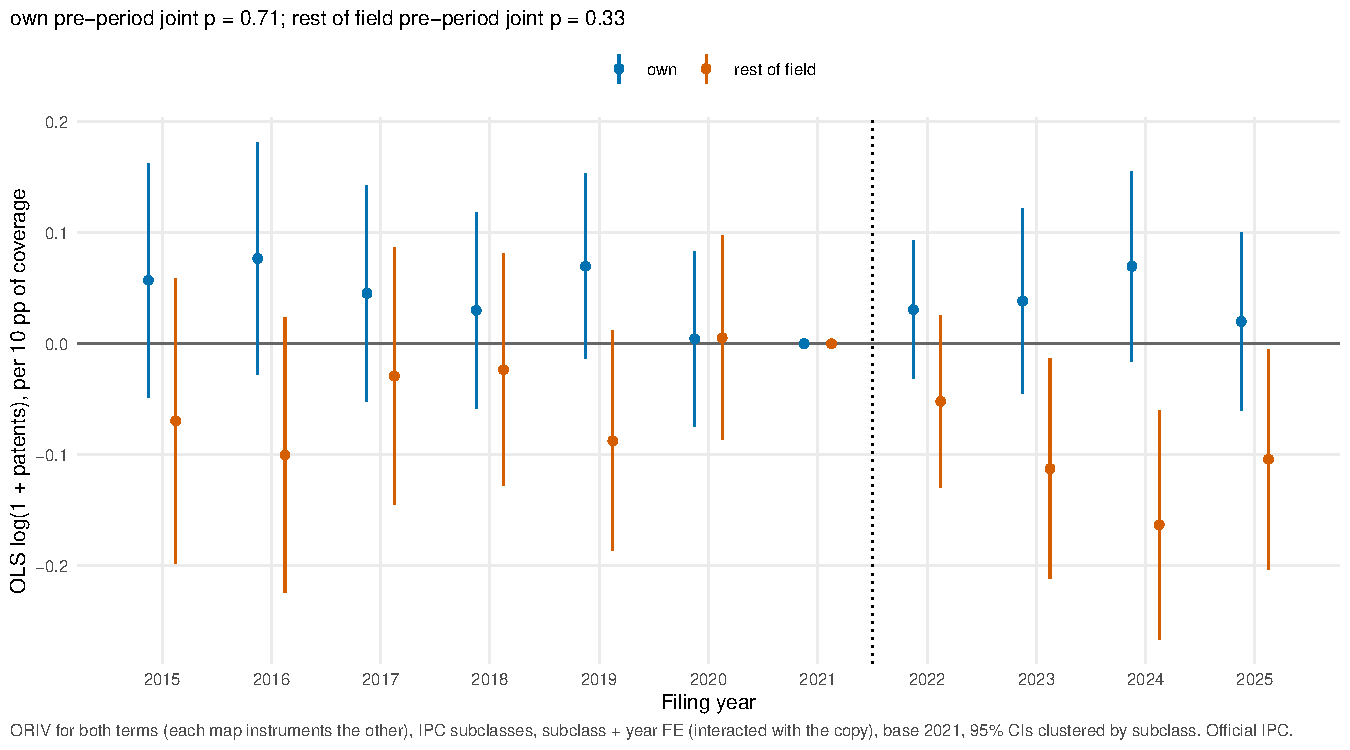
\includegraphics[width=0.78\textwidth]{fig52_oriv_spillovers_es.pdf}
\caption{IPC subclasses: own exposure vs exposure of the rest of the field, both corrected for map noise (ORIV).}
\label{fig:spill}
\end{figure}

\section{The 2014 sanctions}
\label{sec:2014}

The 2014 measures were narrow: an oil-equipment list (at most 4\% of any field's imports), dual-use goods banned for
military end-use, an arms embargo. They coincided with the oil-price collapse, the rouble devaluation and state
import-substitution programmes. Exposure to the dual-use restrictions comes from the Commission's correlation table
(25\% of Western manufactured imports fall in products that \emph{can} be dual-use; 8\% if only fully listed
products count). The most exposed fields are telecommunications, semiconductors, computers, optics and control.

After 2014 the dual-use-exposed fields \emph{gained} relative to others: $+0.072$ per standard deviation in 2014--17
($p=0.01$) and $+0.07$ to $+0.10$ in 2018--21, clearest with the product-name map, whose pre-period is flat (bootstrap
$p=0.77$); with the industry map the rise starts around 2009--11 (Figure~\ref{fig:2014}). The narrow, targeted 2014
restrictions were followed by invention moving \emph{into} the restricted technologies, with strong state support;
the broad 2022 bans were followed by a decline in exposed fields. The 2014 pattern is descriptive: the 2011--2020
State Armament Programme, the devaluation and import-substitution policy favoured the same fields. Adding 2014
dual-use exposure $\times$ year to the 2022 design does not flatten its pre-period and leaves the post-2022 effect at
$-0.08$ to $-0.09$.

\begin{figure}[ht]
\centering
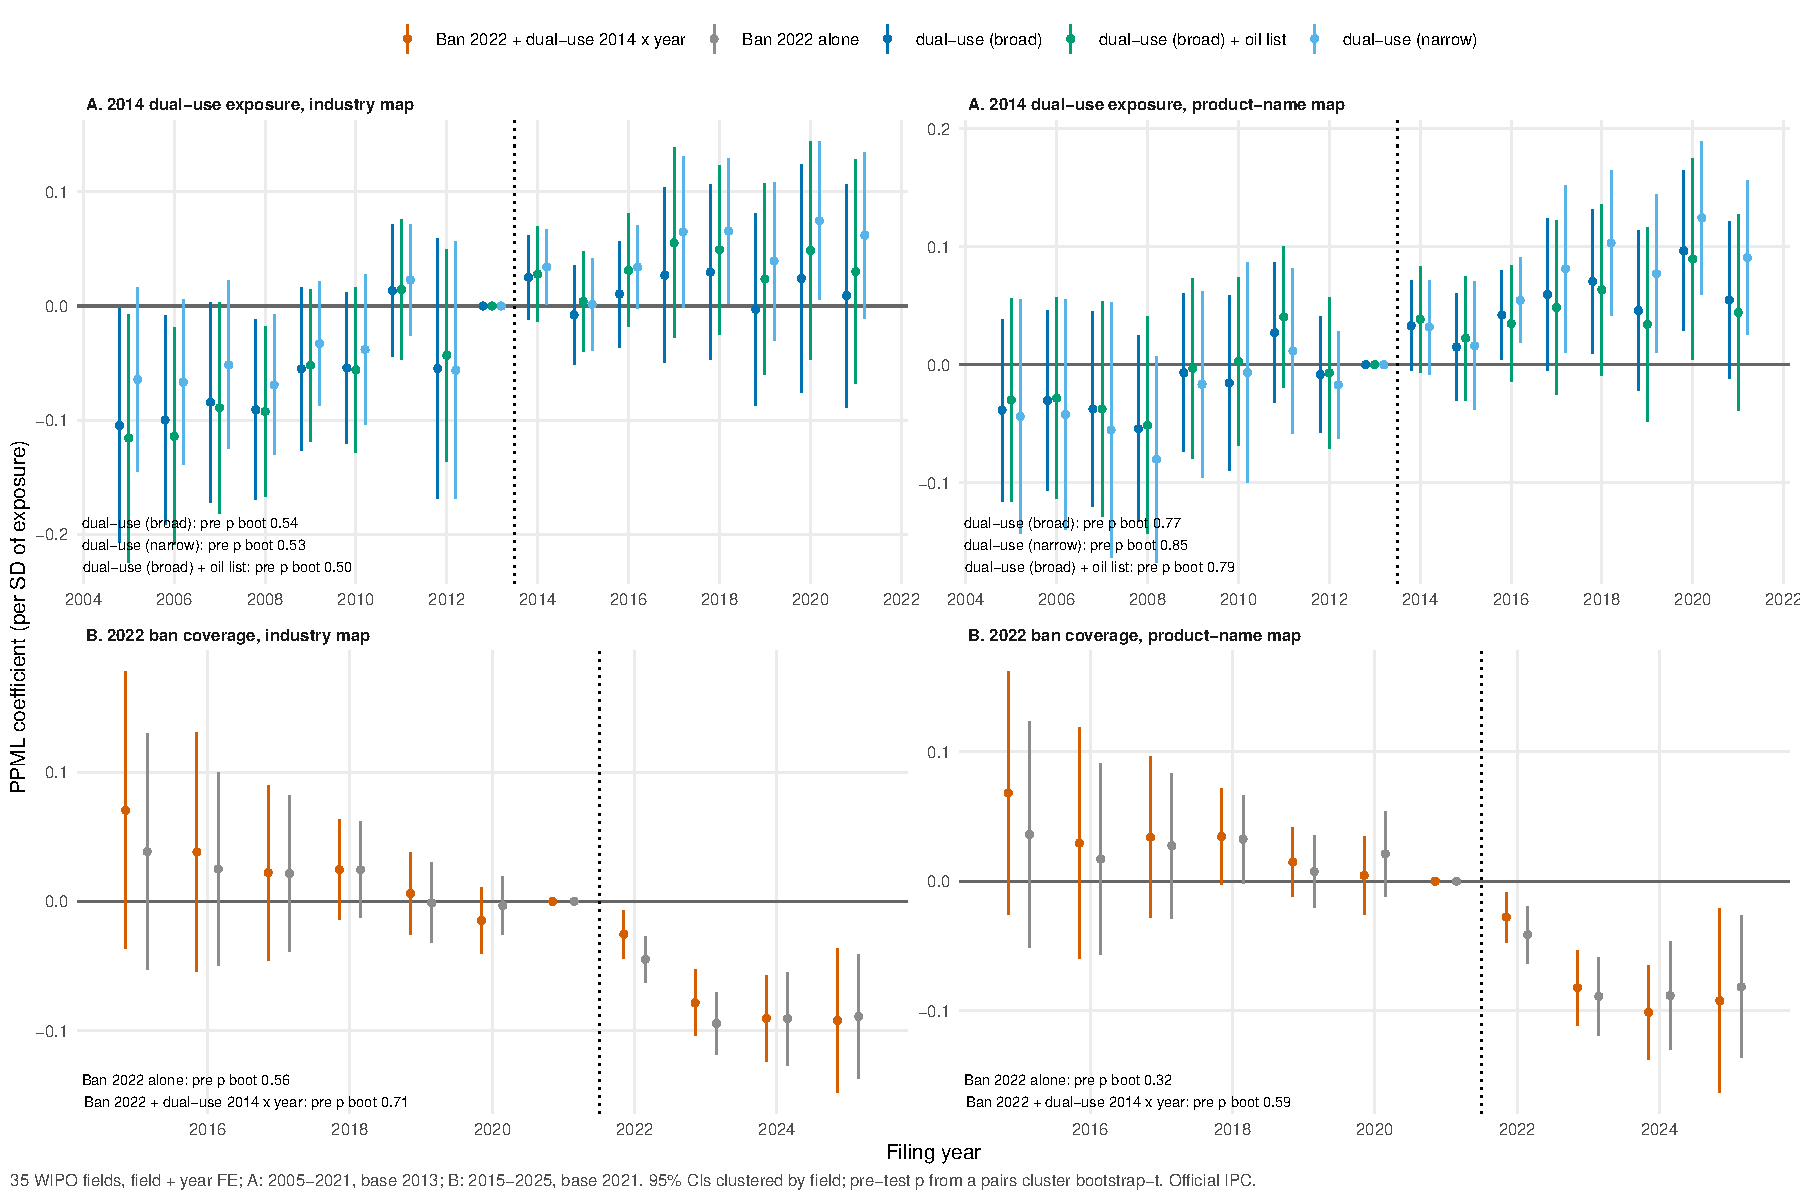
\includegraphics[width=\textwidth]{fig56_dualuse_2014.pdf}
\caption{(A) 2014 dual-use exposure, 2005--2021, base 2013. (B) The 2022 design with and without 2014 dual-use
exposure $\times$ year.}
\label{fig:2014}
\end{figure}

\section{Interpretation}

\begin{enumerate}\setlength\itemsep{0.2em}
  \item \textbf{No import substitution in invention after 2022.} Technologies and industries more exposed to the EU
  bans saw relatively fewer domestic patents, about $-7$ to $-10$\% per standard deviation of exposure. A rise of any
  economically meaningful size is ruled out.
  \item \textbf{The decline is about what was banned.} It holds under four different links between sanctions and
  invention (technology fields; industries by output; by US input weights; by Russia's own 2021 inputs), and Western
  reliance that was not banned shows no effect.
  \item \textbf{It operates at the level of broad technology areas and branches}, and is concentrated in research
  institutes and universities: consistent with lost access to imported equipment, components and Western research
  links (EU--Russia co-publications fell after 2014; \citealp{MakkonenMitze2023}).
  \item \textbf{2014 versus 2022.} Partial, targeted restrictions plus state support coincided with substitution
  into the restricted technologies; a broad cut-off did not.
\end{enumerate}

\paragraph{Caveats.} 2022 is also a shock to military spending, emigration and foreign participation (foreign
filings in Russia halved); field-level comparisons absorb common shocks but not shocks that differ by technology.
About half the field-level contrast comes from the life sciences, where university patenting grew under ministry
targets. Exposure measures rest on concordances (German inventor data for technology $\leftrightarrow$ industry; US
input weights in one version); the EU list stands in for all coalition controls, Annex VII (advanced technology) has
no customs codes, and the general dual-use ban of February 2022 is not yet in the 2022 measure. Patents measure
inventive output, not quality or use. 2025 filings are incomplete.

\section{Next steps}

\begin{enumerate}\setlength\itemsep{0.1em}
  \item Add the general 2022 dual-use ban (Commission correlation table) to 2022 coverage; date electronics from
  February 2022.
  \item Inference for shift-share exposure: permute product-level bans and rebuild exposure
  \citep{AdaoKolesarMorales2019}.
  \item Channels: pre-war Western citation and co-invention shares $\times$ year (knowledge links); China replacement
  by field.
  \item An independent technology $\leftrightarrow$ industry link (text-based or EU-wide) to reduce reliance on the
  German table.
  \item Firm level: patent holders to firms through a name $\to$ tax-ID table, then the Russian Financial Statements
  Database (downloaded, 2011--2025).
\end{enumerate}

\appendix
\section{Additional figures}

\begin{figure}[ht]
\centering
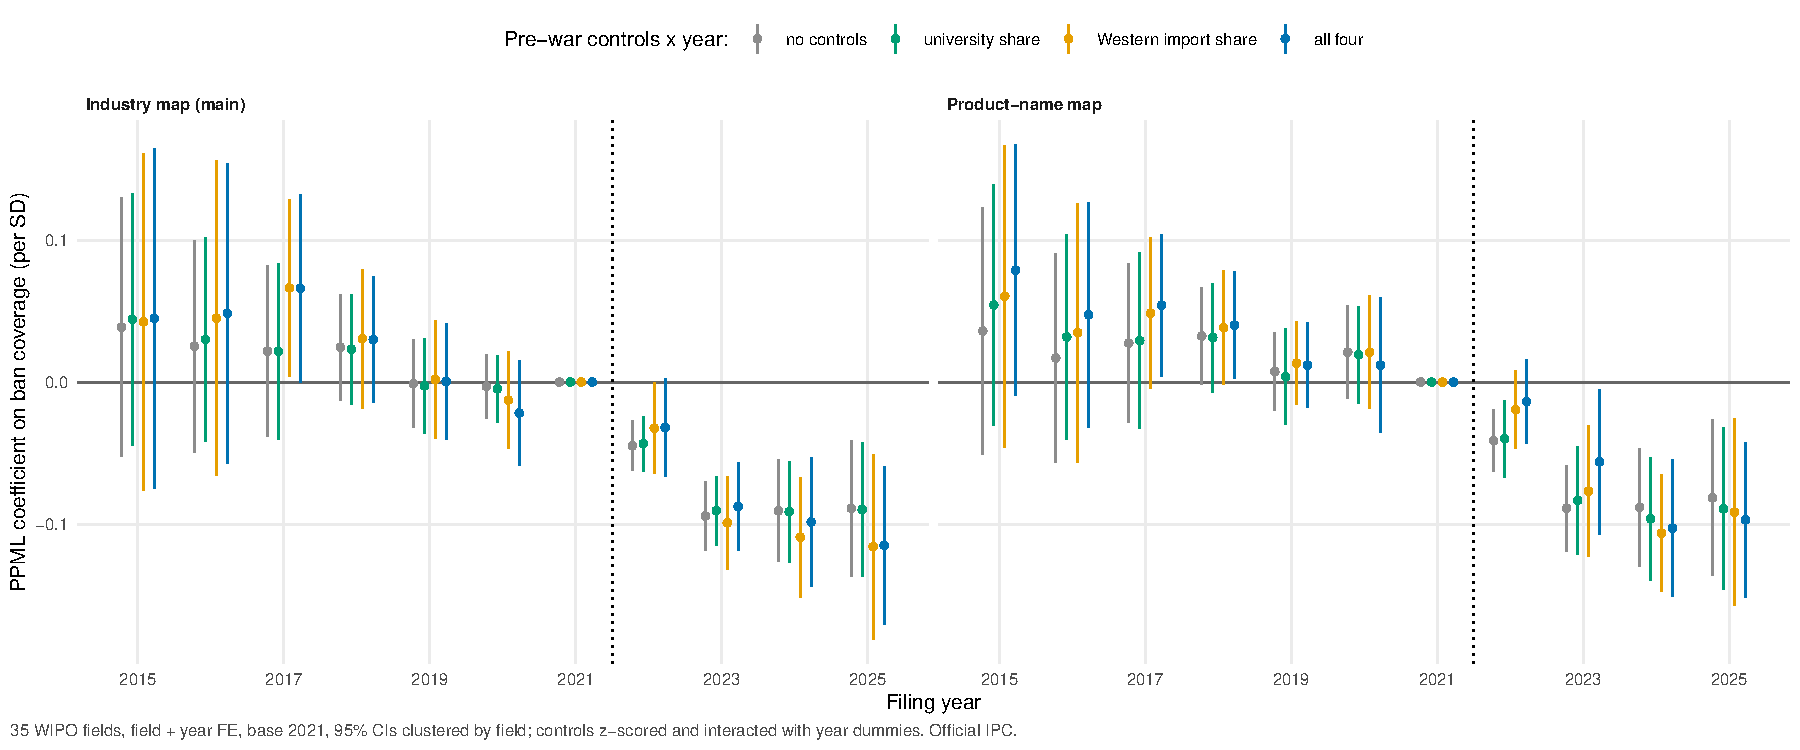
\includegraphics[width=\textwidth]{fig54_prewar_controls_es.pdf}
\caption{Field event study with pre-war characteristics $\times$ year as controls.}
\label{fig:controls}
\end{figure}

\begin{figure}[ht]
\centering
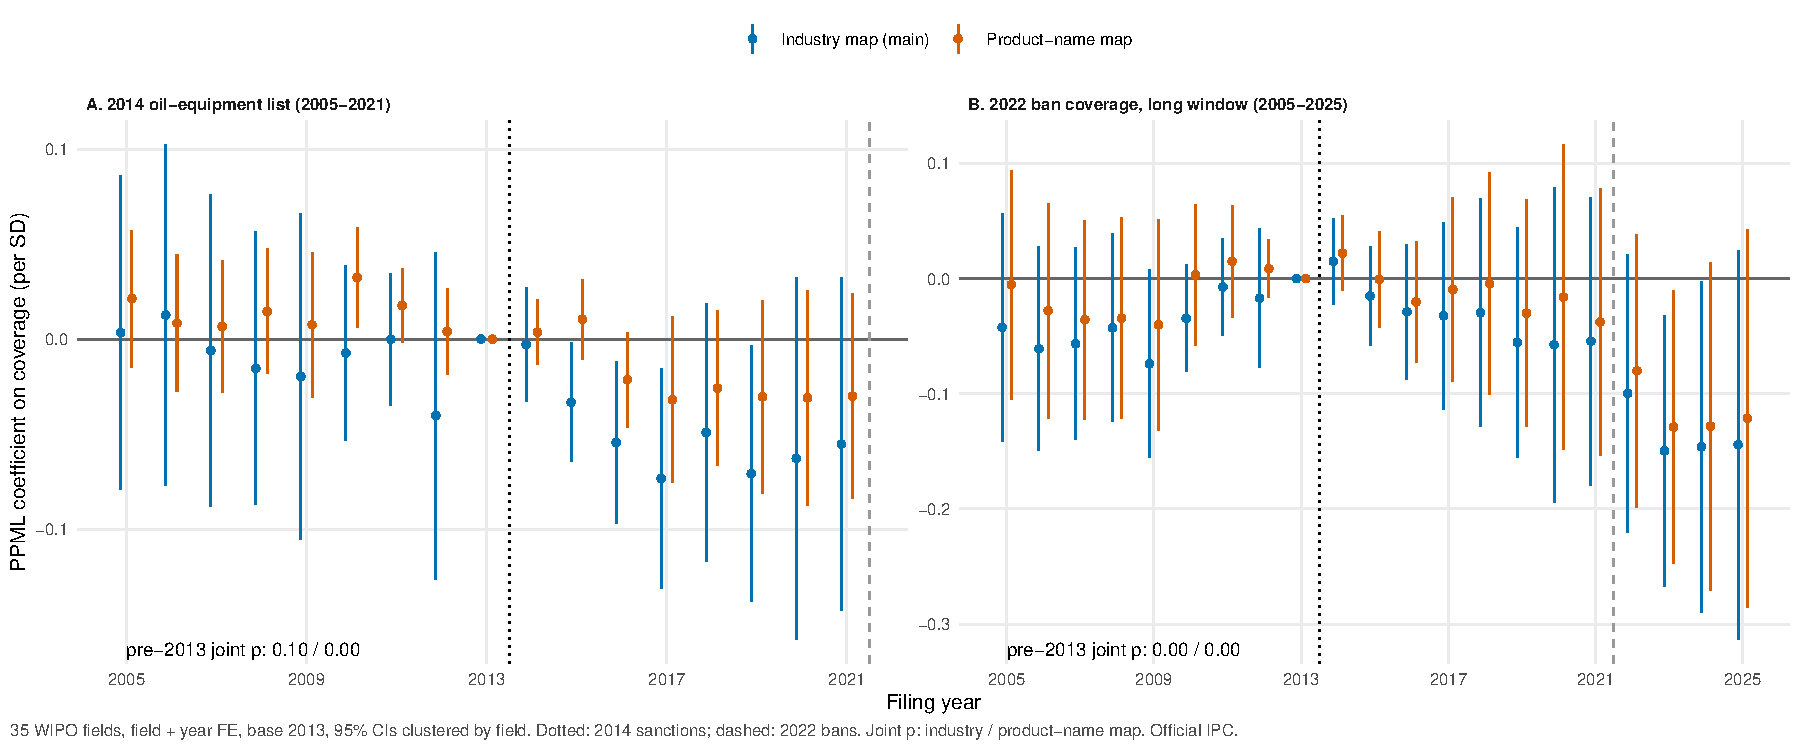
\includegraphics[width=\textwidth]{fig55_2014_official.pdf}
\caption{(A) 2014 oil-equipment list, 2005--2021. (B) 2022 ban coverage over 2005--2025, base 2013.}
\end{figure}

\begin{figure}[ht]
\centering
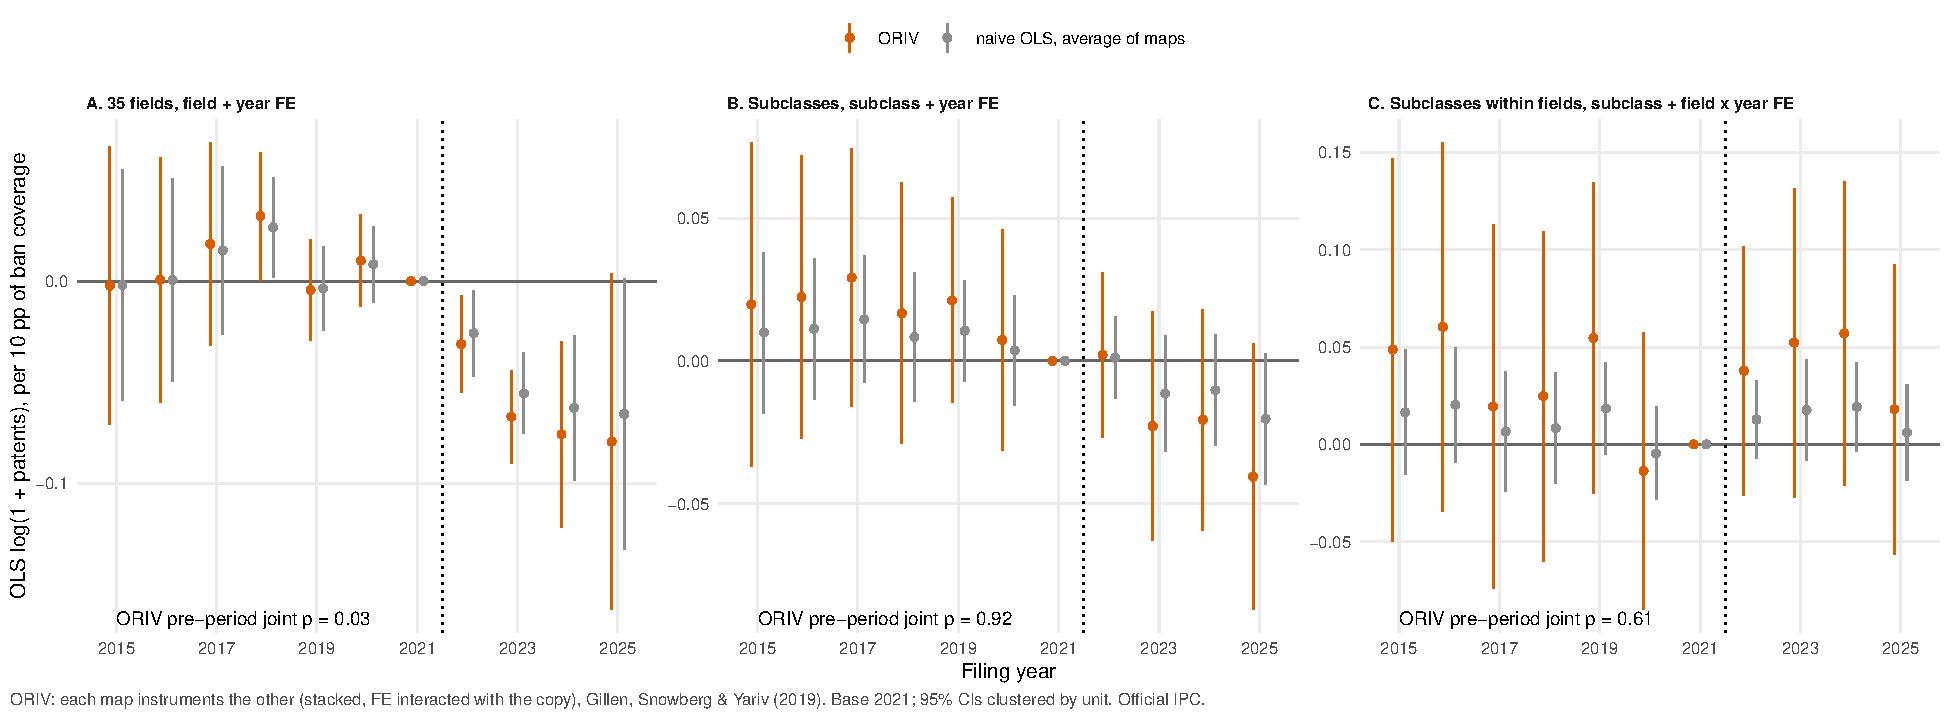
\includegraphics[width=\textwidth]{fig49_oriv_es.pdf}
\caption{ORIV event studies: fields, subclasses across fields, subclasses within fields.}
\end{figure}

\clearpage
\begin{thebibliography}{99}\small
\bibitem[Ad\~{a}o et~al.(2019)]{AdaoKolesarMorales2019}
Ad\~{a}o, R., M.~Koles\'{a}r and E.~Morales (2019). Shift-share designs: Theory and inference. \emph{Quarterly
Journal of Economics} 134(4), 1949--2010.
\bibitem[Borusyak et~al.(2022)]{BorusyakHullJaravel2022}
Borusyak, K., P.~Hull and X.~Jaravel (2022). Quasi-experimental shift-share research designs. \emph{Review of
Economic Studies} 89(1), 181--213.
\bibitem[Dorner and Harhoff(2018)]{DornerHarhoff2018}
Dorner, M. and D.~Harhoff (2018). A novel technology-industry concordance table based on linked
inventor-establishment data. \emph{Research Policy} 47(4), 768--781. Tables from IAB FDZ Methodenreport 07/2017.
\bibitem[Egorov et~al.(2026)]{EgorovEtAl2026}
Egorov, K., V.~Korovkin, A.~Makarin and D.~Nigmatulina (2026). Export sanctions: Rerouting, disruption, and the
reach of economic warfare. Working paper, July 2026.
\bibitem[Gaulier and Zignago(2010)]{GaulierZignago2010}
Gaulier, G. and S.~Zignago (2010). BACI: International trade database at the product-level. CEPII Working Paper
2010-23.
\bibitem[Gillen et~al.(2019)]{GillenSnowbergYariv2019}
Gillen, B., E.~Snowberg and L.~Yariv (2019). Experimenting with measurement error: Techniques with applications to
the Caltech cohort study. \emph{Journal of Political Economy} 127(4), 1826--1863.
\bibitem[Makkonen and Mitze(2023)]{MakkonenMitze2023}
Makkonen, T. and T.~Mitze (2023). Geo-political conflicts, economic sanctions and international knowledge flows.
\emph{The World Economy} 46(10), 2926--2949.
\bibitem[Rambachan and Roth(2023)]{RambachanRoth2023}
Rambachan, A. and J.~Roth (2023). A more credible approach to parallel trends. \emph{Review of Economic Studies}
90(5), 2555--2591.
\end{thebibliography}

\end{document}
